The algorithm can be implemented using the following python code snippet: \\
\begin{lstlisting}
    import numpy as np
    
    A = 0
    
    N = 100000
    for _ in range(N):
        x = np.random.uniform(-1, 1)
        y = np.random.uniform(-1, 1)
        if x**2 + y**2 <= 1:
            A += 1
    
    z = 4 * A / N
    print(z) \end{lstlisting}
With this, a value for $\pi$ can be estimated, running the above code 
returns $3.14312$. The ratio of $A$ to $N$ is 
directly proportional to another ratio, namely that of a the area of a 
unit circle to the area of a square with side length 2. One could thus 
in principle calculate $\pi$ by e.g. throwing darts onto a square surface with 
a circle drawn on it. This is because the number of "hits" can be 
assumed to be proportional to the hit probability, which again is directly 
proportional to the respective area. This method can only work if the 
distribution of random numbers is uniform and $N$ is large enough. \\
\\
Visualization:
\begin{figure}[h!]
    \centering
    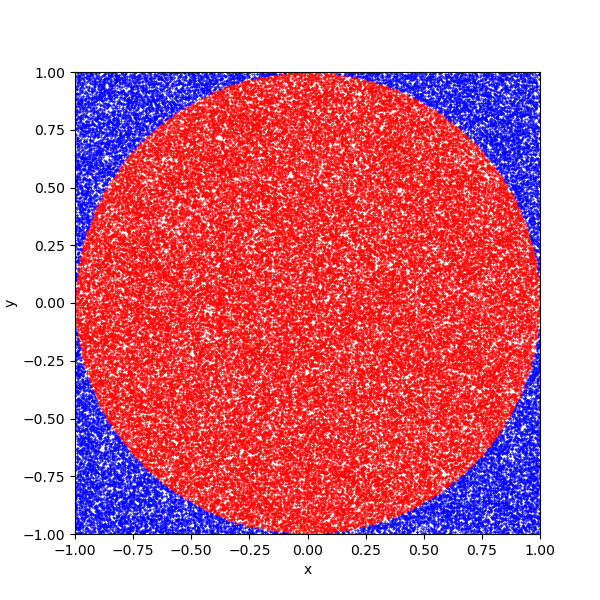
\includegraphics[width=.6\textwidth]{./figures/task_03_N100000.png}
\end{figure} \ \\ 
